\documentclass[tikz,border=7mm]{standalone}
\usepackage[T1]{fontenc}
\usepackage[utf8]{inputenc}
\usepackage{lmodern}
\usepackage{amsmath}
\usepackage{xcolor}
\usetikzlibrary{arrows.meta,calc,positioning}
\definecolor{TitleBlue}{HTML}{1D4F91}
\definecolor{ElecBlue}{HTML}{1F6FFF}
\definecolor{Grid}{HTML}{6F7D89}
\definecolor{Dark}{HTML}{344250}
\definecolor{SoftGray}{HTML}{F7F9FC}
\definecolor{ZeroBorder}{HTML}{1F6FFF}
\definecolor{GoodGreen}{HTML}{5D8F00}
\definecolor{Bank0}{HTML}{BFD7F0}
\definecolor{Bank1}{HTML}{C9E3C0}
\definecolor{Bank2}{HTML}{F2E4A7}
\definecolor{Bank3}{HTML}{F1C9A9}
\definecolor{Bank4}{HTML}{D7BEE9}
\definecolor{Bank5}{HTML}{E9C5DA}
\definecolor{Bank6}{HTML}{C7E6E8}
\definecolor{Bank7}{HTML}{F2C4CF}
\begin{document}
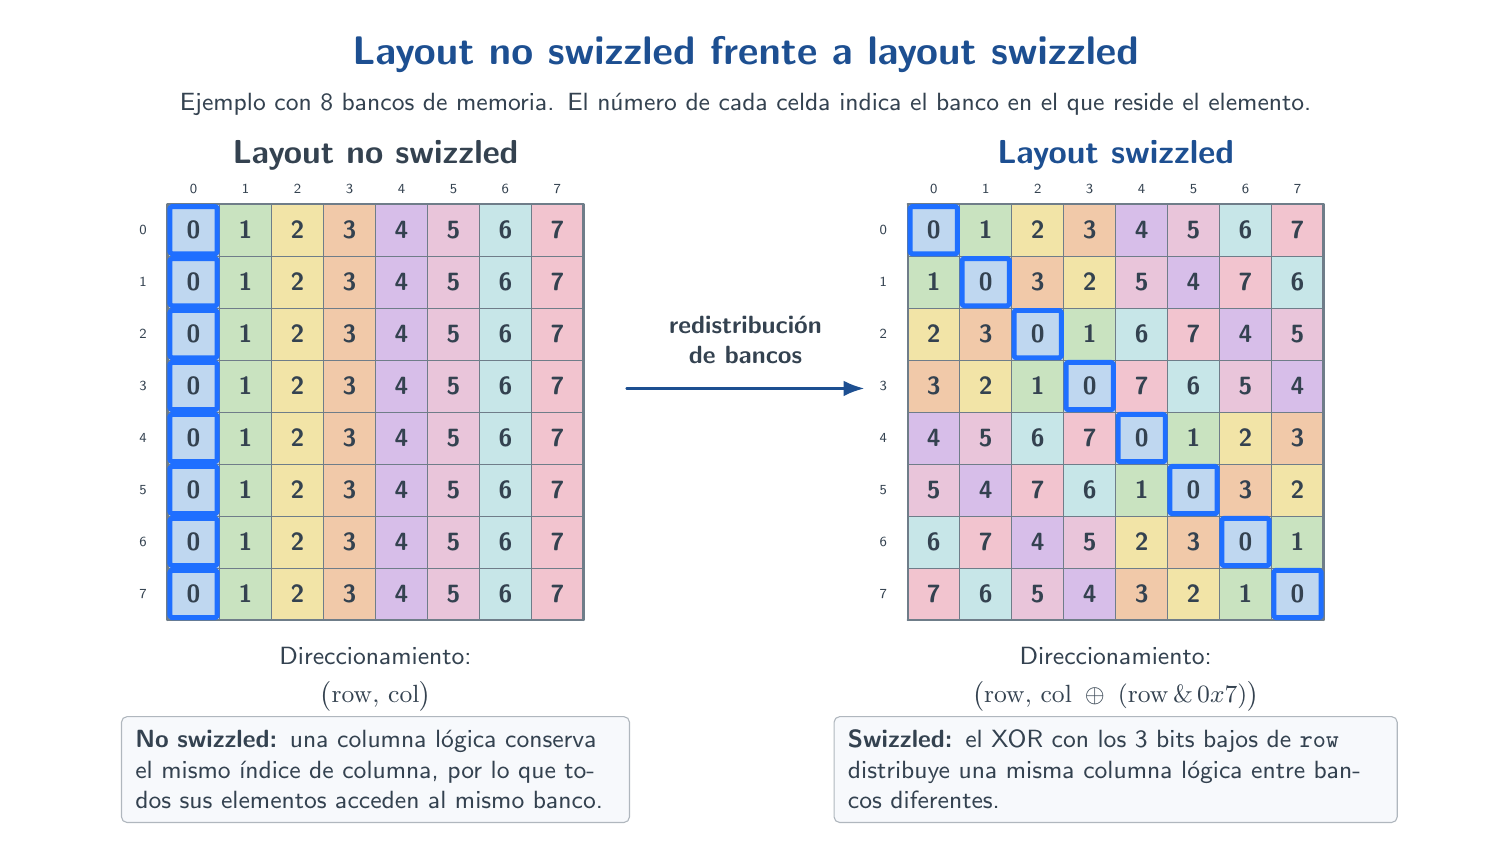
\begin{tikzpicture}[x=1cm,y=1cm,line cap=round,line join=round,>={Latex[length=2.2mm,width=1.6mm]}]
\node[font=\sffamily\bfseries\Large,text=TitleBlue,align=center,text width=18cm] at (8.590,9.55) {Layout no \emph{swizzled} frente a layout \emph{swizzled}};
\node[font=\sffamily\small,text=Dark,align=center,text width=17.5cm] at (8.590,8.92) {Ejemplo con 8 bancos de memoria. El número de cada celda indica el banco en el que reside el elemento.};
\node[font=\sffamily\bfseries\large,text=Dark] at (3.890,8.270) {Layout no \emph{swizzled}};
\node[font=\sffamily\bfseries\large,text=TitleBlue] at (13.290,8.270) {Layout \emph{swizzled}};
\node[font=\sffamily\tiny,text=Dark] at (1.580,7.850) {0};
\node[font=\sffamily\tiny,text=Dark] at (10.980,7.850) {0};
\node[font=\sffamily\tiny,text=Dark] at (2.240,7.850) {1};
\node[font=\sffamily\tiny,text=Dark] at (11.640,7.850) {1};
\node[font=\sffamily\tiny,text=Dark] at (2.900,7.850) {2};
\node[font=\sffamily\tiny,text=Dark] at (12.300,7.850) {2};
\node[font=\sffamily\tiny,text=Dark] at (3.560,7.850) {3};
\node[font=\sffamily\tiny,text=Dark] at (12.960,7.850) {3};
\node[font=\sffamily\tiny,text=Dark] at (4.220,7.850) {4};
\node[font=\sffamily\tiny,text=Dark] at (13.620,7.850) {4};
\node[font=\sffamily\tiny,text=Dark] at (4.880,7.850) {5};
\node[font=\sffamily\tiny,text=Dark] at (14.280,7.850) {5};
\node[font=\sffamily\tiny,text=Dark] at (5.540,7.850) {6};
\node[font=\sffamily\tiny,text=Dark] at (14.940,7.850) {6};
\node[font=\sffamily\tiny,text=Dark] at (6.200,7.850) {7};
\node[font=\sffamily\tiny,text=Dark] at (15.600,7.850) {7};
\node[anchor=east,font=\sffamily\tiny,text=Dark] at (1.110,7.320) {0};
\node[anchor=east,font=\sffamily\tiny,text=Dark] at (10.510,7.320) {0};
\node[anchor=east,font=\sffamily\tiny,text=Dark] at (1.110,6.660) {1};
\node[anchor=east,font=\sffamily\tiny,text=Dark] at (10.510,6.660) {1};
\node[anchor=east,font=\sffamily\tiny,text=Dark] at (1.110,6.000) {2};
\node[anchor=east,font=\sffamily\tiny,text=Dark] at (10.510,6.000) {2};
\node[anchor=east,font=\sffamily\tiny,text=Dark] at (1.110,5.340) {3};
\node[anchor=east,font=\sffamily\tiny,text=Dark] at (10.510,5.340) {3};
\node[anchor=east,font=\sffamily\tiny,text=Dark] at (1.110,4.680) {4};
\node[anchor=east,font=\sffamily\tiny,text=Dark] at (10.510,4.680) {4};
\node[anchor=east,font=\sffamily\tiny,text=Dark] at (1.110,4.020) {5};
\node[anchor=east,font=\sffamily\tiny,text=Dark] at (10.510,4.020) {5};
\node[anchor=east,font=\sffamily\tiny,text=Dark] at (1.110,3.360) {6};
\node[anchor=east,font=\sffamily\tiny,text=Dark] at (10.510,3.360) {6};
\node[anchor=east,font=\sffamily\tiny,text=Dark] at (1.110,2.700) {7};
\node[anchor=east,font=\sffamily\tiny,text=Dark] at (10.510,2.700) {7};
\fill[Bank0] (1.250,7.650) rectangle (1.910,6.990);
\fill[Bank0] (10.650,7.650) rectangle (11.310,6.990);
\node[font=\sffamily\small\bfseries,text=Dark] at (1.580,7.320) {0};
\node[font=\sffamily\small\bfseries,text=Dark] at (10.980,7.320) {0};
\fill[Bank1] (1.910,7.650) rectangle (2.570,6.990);
\fill[Bank1] (11.310,7.650) rectangle (11.970,6.990);
\node[font=\sffamily\small\bfseries,text=Dark] at (2.240,7.320) {1};
\node[font=\sffamily\small\bfseries,text=Dark] at (11.640,7.320) {1};
\fill[Bank2] (2.570,7.650) rectangle (3.230,6.990);
\fill[Bank2] (11.970,7.650) rectangle (12.630,6.990);
\node[font=\sffamily\small\bfseries,text=Dark] at (2.900,7.320) {2};
\node[font=\sffamily\small\bfseries,text=Dark] at (12.300,7.320) {2};
\fill[Bank3] (3.230,7.650) rectangle (3.890,6.990);
\fill[Bank3] (12.630,7.650) rectangle (13.290,6.990);
\node[font=\sffamily\small\bfseries,text=Dark] at (3.560,7.320) {3};
\node[font=\sffamily\small\bfseries,text=Dark] at (12.960,7.320) {3};
\fill[Bank4] (3.890,7.650) rectangle (4.550,6.990);
\fill[Bank4] (13.290,7.650) rectangle (13.950,6.990);
\node[font=\sffamily\small\bfseries,text=Dark] at (4.220,7.320) {4};
\node[font=\sffamily\small\bfseries,text=Dark] at (13.620,7.320) {4};
\fill[Bank5] (4.550,7.650) rectangle (5.210,6.990);
\fill[Bank5] (13.950,7.650) rectangle (14.610,6.990);
\node[font=\sffamily\small\bfseries,text=Dark] at (4.880,7.320) {5};
\node[font=\sffamily\small\bfseries,text=Dark] at (14.280,7.320) {5};
\fill[Bank6] (5.210,7.650) rectangle (5.870,6.990);
\fill[Bank6] (14.610,7.650) rectangle (15.270,6.990);
\node[font=\sffamily\small\bfseries,text=Dark] at (5.540,7.320) {6};
\node[font=\sffamily\small\bfseries,text=Dark] at (14.940,7.320) {6};
\fill[Bank7] (5.870,7.650) rectangle (6.530,6.990);
\fill[Bank7] (15.270,7.650) rectangle (15.930,6.990);
\node[font=\sffamily\small\bfseries,text=Dark] at (6.200,7.320) {7};
\node[font=\sffamily\small\bfseries,text=Dark] at (15.600,7.320) {7};
\fill[Bank0] (1.250,6.990) rectangle (1.910,6.330);
\fill[Bank1] (10.650,6.990) rectangle (11.310,6.330);
\node[font=\sffamily\small\bfseries,text=Dark] at (1.580,6.660) {0};
\node[font=\sffamily\small\bfseries,text=Dark] at (10.980,6.660) {1};
\fill[Bank1] (1.910,6.990) rectangle (2.570,6.330);
\fill[Bank0] (11.310,6.990) rectangle (11.970,6.330);
\node[font=\sffamily\small\bfseries,text=Dark] at (2.240,6.660) {1};
\node[font=\sffamily\small\bfseries,text=Dark] at (11.640,6.660) {0};
\fill[Bank2] (2.570,6.990) rectangle (3.230,6.330);
\fill[Bank3] (11.970,6.990) rectangle (12.630,6.330);
\node[font=\sffamily\small\bfseries,text=Dark] at (2.900,6.660) {2};
\node[font=\sffamily\small\bfseries,text=Dark] at (12.300,6.660) {3};
\fill[Bank3] (3.230,6.990) rectangle (3.890,6.330);
\fill[Bank2] (12.630,6.990) rectangle (13.290,6.330);
\node[font=\sffamily\small\bfseries,text=Dark] at (3.560,6.660) {3};
\node[font=\sffamily\small\bfseries,text=Dark] at (12.960,6.660) {2};
\fill[Bank4] (3.890,6.990) rectangle (4.550,6.330);
\fill[Bank5] (13.290,6.990) rectangle (13.950,6.330);
\node[font=\sffamily\small\bfseries,text=Dark] at (4.220,6.660) {4};
\node[font=\sffamily\small\bfseries,text=Dark] at (13.620,6.660) {5};
\fill[Bank5] (4.550,6.990) rectangle (5.210,6.330);
\fill[Bank4] (13.950,6.990) rectangle (14.610,6.330);
\node[font=\sffamily\small\bfseries,text=Dark] at (4.880,6.660) {5};
\node[font=\sffamily\small\bfseries,text=Dark] at (14.280,6.660) {4};
\fill[Bank6] (5.210,6.990) rectangle (5.870,6.330);
\fill[Bank7] (14.610,6.990) rectangle (15.270,6.330);
\node[font=\sffamily\small\bfseries,text=Dark] at (5.540,6.660) {6};
\node[font=\sffamily\small\bfseries,text=Dark] at (14.940,6.660) {7};
\fill[Bank7] (5.870,6.990) rectangle (6.530,6.330);
\fill[Bank6] (15.270,6.990) rectangle (15.930,6.330);
\node[font=\sffamily\small\bfseries,text=Dark] at (6.200,6.660) {7};
\node[font=\sffamily\small\bfseries,text=Dark] at (15.600,6.660) {6};
\fill[Bank0] (1.250,6.330) rectangle (1.910,5.670);
\fill[Bank2] (10.650,6.330) rectangle (11.310,5.670);
\node[font=\sffamily\small\bfseries,text=Dark] at (1.580,6.000) {0};
\node[font=\sffamily\small\bfseries,text=Dark] at (10.980,6.000) {2};
\fill[Bank1] (1.910,6.330) rectangle (2.570,5.670);
\fill[Bank3] (11.310,6.330) rectangle (11.970,5.670);
\node[font=\sffamily\small\bfseries,text=Dark] at (2.240,6.000) {1};
\node[font=\sffamily\small\bfseries,text=Dark] at (11.640,6.000) {3};
\fill[Bank2] (2.570,6.330) rectangle (3.230,5.670);
\fill[Bank0] (11.970,6.330) rectangle (12.630,5.670);
\node[font=\sffamily\small\bfseries,text=Dark] at (2.900,6.000) {2};
\node[font=\sffamily\small\bfseries,text=Dark] at (12.300,6.000) {0};
\fill[Bank3] (3.230,6.330) rectangle (3.890,5.670);
\fill[Bank1] (12.630,6.330) rectangle (13.290,5.670);
\node[font=\sffamily\small\bfseries,text=Dark] at (3.560,6.000) {3};
\node[font=\sffamily\small\bfseries,text=Dark] at (12.960,6.000) {1};
\fill[Bank4] (3.890,6.330) rectangle (4.550,5.670);
\fill[Bank6] (13.290,6.330) rectangle (13.950,5.670);
\node[font=\sffamily\small\bfseries,text=Dark] at (4.220,6.000) {4};
\node[font=\sffamily\small\bfseries,text=Dark] at (13.620,6.000) {6};
\fill[Bank5] (4.550,6.330) rectangle (5.210,5.670);
\fill[Bank7] (13.950,6.330) rectangle (14.610,5.670);
\node[font=\sffamily\small\bfseries,text=Dark] at (4.880,6.000) {5};
\node[font=\sffamily\small\bfseries,text=Dark] at (14.280,6.000) {7};
\fill[Bank6] (5.210,6.330) rectangle (5.870,5.670);
\fill[Bank4] (14.610,6.330) rectangle (15.270,5.670);
\node[font=\sffamily\small\bfseries,text=Dark] at (5.540,6.000) {6};
\node[font=\sffamily\small\bfseries,text=Dark] at (14.940,6.000) {4};
\fill[Bank7] (5.870,6.330) rectangle (6.530,5.670);
\fill[Bank5] (15.270,6.330) rectangle (15.930,5.670);
\node[font=\sffamily\small\bfseries,text=Dark] at (6.200,6.000) {7};
\node[font=\sffamily\small\bfseries,text=Dark] at (15.600,6.000) {5};
\fill[Bank0] (1.250,5.670) rectangle (1.910,5.010);
\fill[Bank3] (10.650,5.670) rectangle (11.310,5.010);
\node[font=\sffamily\small\bfseries,text=Dark] at (1.580,5.340) {0};
\node[font=\sffamily\small\bfseries,text=Dark] at (10.980,5.340) {3};
\fill[Bank1] (1.910,5.670) rectangle (2.570,5.010);
\fill[Bank2] (11.310,5.670) rectangle (11.970,5.010);
\node[font=\sffamily\small\bfseries,text=Dark] at (2.240,5.340) {1};
\node[font=\sffamily\small\bfseries,text=Dark] at (11.640,5.340) {2};
\fill[Bank2] (2.570,5.670) rectangle (3.230,5.010);
\fill[Bank1] (11.970,5.670) rectangle (12.630,5.010);
\node[font=\sffamily\small\bfseries,text=Dark] at (2.900,5.340) {2};
\node[font=\sffamily\small\bfseries,text=Dark] at (12.300,5.340) {1};
\fill[Bank3] (3.230,5.670) rectangle (3.890,5.010);
\fill[Bank0] (12.630,5.670) rectangle (13.290,5.010);
\node[font=\sffamily\small\bfseries,text=Dark] at (3.560,5.340) {3};
\node[font=\sffamily\small\bfseries,text=Dark] at (12.960,5.340) {0};
\fill[Bank4] (3.890,5.670) rectangle (4.550,5.010);
\fill[Bank7] (13.290,5.670) rectangle (13.950,5.010);
\node[font=\sffamily\small\bfseries,text=Dark] at (4.220,5.340) {4};
\node[font=\sffamily\small\bfseries,text=Dark] at (13.620,5.340) {7};
\fill[Bank5] (4.550,5.670) rectangle (5.210,5.010);
\fill[Bank6] (13.950,5.670) rectangle (14.610,5.010);
\node[font=\sffamily\small\bfseries,text=Dark] at (4.880,5.340) {5};
\node[font=\sffamily\small\bfseries,text=Dark] at (14.280,5.340) {6};
\fill[Bank6] (5.210,5.670) rectangle (5.870,5.010);
\fill[Bank5] (14.610,5.670) rectangle (15.270,5.010);
\node[font=\sffamily\small\bfseries,text=Dark] at (5.540,5.340) {6};
\node[font=\sffamily\small\bfseries,text=Dark] at (14.940,5.340) {5};
\fill[Bank7] (5.870,5.670) rectangle (6.530,5.010);
\fill[Bank4] (15.270,5.670) rectangle (15.930,5.010);
\node[font=\sffamily\small\bfseries,text=Dark] at (6.200,5.340) {7};
\node[font=\sffamily\small\bfseries,text=Dark] at (15.600,5.340) {4};
\fill[Bank0] (1.250,5.010) rectangle (1.910,4.350);
\fill[Bank4] (10.650,5.010) rectangle (11.310,4.350);
\node[font=\sffamily\small\bfseries,text=Dark] at (1.580,4.680) {0};
\node[font=\sffamily\small\bfseries,text=Dark] at (10.980,4.680) {4};
\fill[Bank1] (1.910,5.010) rectangle (2.570,4.350);
\fill[Bank5] (11.310,5.010) rectangle (11.970,4.350);
\node[font=\sffamily\small\bfseries,text=Dark] at (2.240,4.680) {1};
\node[font=\sffamily\small\bfseries,text=Dark] at (11.640,4.680) {5};
\fill[Bank2] (2.570,5.010) rectangle (3.230,4.350);
\fill[Bank6] (11.970,5.010) rectangle (12.630,4.350);
\node[font=\sffamily\small\bfseries,text=Dark] at (2.900,4.680) {2};
\node[font=\sffamily\small\bfseries,text=Dark] at (12.300,4.680) {6};
\fill[Bank3] (3.230,5.010) rectangle (3.890,4.350);
\fill[Bank7] (12.630,5.010) rectangle (13.290,4.350);
\node[font=\sffamily\small\bfseries,text=Dark] at (3.560,4.680) {3};
\node[font=\sffamily\small\bfseries,text=Dark] at (12.960,4.680) {7};
\fill[Bank4] (3.890,5.010) rectangle (4.550,4.350);
\fill[Bank0] (13.290,5.010) rectangle (13.950,4.350);
\node[font=\sffamily\small\bfseries,text=Dark] at (4.220,4.680) {4};
\node[font=\sffamily\small\bfseries,text=Dark] at (13.620,4.680) {0};
\fill[Bank5] (4.550,5.010) rectangle (5.210,4.350);
\fill[Bank1] (13.950,5.010) rectangle (14.610,4.350);
\node[font=\sffamily\small\bfseries,text=Dark] at (4.880,4.680) {5};
\node[font=\sffamily\small\bfseries,text=Dark] at (14.280,4.680) {1};
\fill[Bank6] (5.210,5.010) rectangle (5.870,4.350);
\fill[Bank2] (14.610,5.010) rectangle (15.270,4.350);
\node[font=\sffamily\small\bfseries,text=Dark] at (5.540,4.680) {6};
\node[font=\sffamily\small\bfseries,text=Dark] at (14.940,4.680) {2};
\fill[Bank7] (5.870,5.010) rectangle (6.530,4.350);
\fill[Bank3] (15.270,5.010) rectangle (15.930,4.350);
\node[font=\sffamily\small\bfseries,text=Dark] at (6.200,4.680) {7};
\node[font=\sffamily\small\bfseries,text=Dark] at (15.600,4.680) {3};
\fill[Bank0] (1.250,4.350) rectangle (1.910,3.690);
\fill[Bank5] (10.650,4.350) rectangle (11.310,3.690);
\node[font=\sffamily\small\bfseries,text=Dark] at (1.580,4.020) {0};
\node[font=\sffamily\small\bfseries,text=Dark] at (10.980,4.020) {5};
\fill[Bank1] (1.910,4.350) rectangle (2.570,3.690);
\fill[Bank4] (11.310,4.350) rectangle (11.970,3.690);
\node[font=\sffamily\small\bfseries,text=Dark] at (2.240,4.020) {1};
\node[font=\sffamily\small\bfseries,text=Dark] at (11.640,4.020) {4};
\fill[Bank2] (2.570,4.350) rectangle (3.230,3.690);
\fill[Bank7] (11.970,4.350) rectangle (12.630,3.690);
\node[font=\sffamily\small\bfseries,text=Dark] at (2.900,4.020) {2};
\node[font=\sffamily\small\bfseries,text=Dark] at (12.300,4.020) {7};
\fill[Bank3] (3.230,4.350) rectangle (3.890,3.690);
\fill[Bank6] (12.630,4.350) rectangle (13.290,3.690);
\node[font=\sffamily\small\bfseries,text=Dark] at (3.560,4.020) {3};
\node[font=\sffamily\small\bfseries,text=Dark] at (12.960,4.020) {6};
\fill[Bank4] (3.890,4.350) rectangle (4.550,3.690);
\fill[Bank1] (13.290,4.350) rectangle (13.950,3.690);
\node[font=\sffamily\small\bfseries,text=Dark] at (4.220,4.020) {4};
\node[font=\sffamily\small\bfseries,text=Dark] at (13.620,4.020) {1};
\fill[Bank5] (4.550,4.350) rectangle (5.210,3.690);
\fill[Bank0] (13.950,4.350) rectangle (14.610,3.690);
\node[font=\sffamily\small\bfseries,text=Dark] at (4.880,4.020) {5};
\node[font=\sffamily\small\bfseries,text=Dark] at (14.280,4.020) {0};
\fill[Bank6] (5.210,4.350) rectangle (5.870,3.690);
\fill[Bank3] (14.610,4.350) rectangle (15.270,3.690);
\node[font=\sffamily\small\bfseries,text=Dark] at (5.540,4.020) {6};
\node[font=\sffamily\small\bfseries,text=Dark] at (14.940,4.020) {3};
\fill[Bank7] (5.870,4.350) rectangle (6.530,3.690);
\fill[Bank2] (15.270,4.350) rectangle (15.930,3.690);
\node[font=\sffamily\small\bfseries,text=Dark] at (6.200,4.020) {7};
\node[font=\sffamily\small\bfseries,text=Dark] at (15.600,4.020) {2};
\fill[Bank0] (1.250,3.690) rectangle (1.910,3.030);
\fill[Bank6] (10.650,3.690) rectangle (11.310,3.030);
\node[font=\sffamily\small\bfseries,text=Dark] at (1.580,3.360) {0};
\node[font=\sffamily\small\bfseries,text=Dark] at (10.980,3.360) {6};
\fill[Bank1] (1.910,3.690) rectangle (2.570,3.030);
\fill[Bank7] (11.310,3.690) rectangle (11.970,3.030);
\node[font=\sffamily\small\bfseries,text=Dark] at (2.240,3.360) {1};
\node[font=\sffamily\small\bfseries,text=Dark] at (11.640,3.360) {7};
\fill[Bank2] (2.570,3.690) rectangle (3.230,3.030);
\fill[Bank4] (11.970,3.690) rectangle (12.630,3.030);
\node[font=\sffamily\small\bfseries,text=Dark] at (2.900,3.360) {2};
\node[font=\sffamily\small\bfseries,text=Dark] at (12.300,3.360) {4};
\fill[Bank3] (3.230,3.690) rectangle (3.890,3.030);
\fill[Bank5] (12.630,3.690) rectangle (13.290,3.030);
\node[font=\sffamily\small\bfseries,text=Dark] at (3.560,3.360) {3};
\node[font=\sffamily\small\bfseries,text=Dark] at (12.960,3.360) {5};
\fill[Bank4] (3.890,3.690) rectangle (4.550,3.030);
\fill[Bank2] (13.290,3.690) rectangle (13.950,3.030);
\node[font=\sffamily\small\bfseries,text=Dark] at (4.220,3.360) {4};
\node[font=\sffamily\small\bfseries,text=Dark] at (13.620,3.360) {2};
\fill[Bank5] (4.550,3.690) rectangle (5.210,3.030);
\fill[Bank3] (13.950,3.690) rectangle (14.610,3.030);
\node[font=\sffamily\small\bfseries,text=Dark] at (4.880,3.360) {5};
\node[font=\sffamily\small\bfseries,text=Dark] at (14.280,3.360) {3};
\fill[Bank6] (5.210,3.690) rectangle (5.870,3.030);
\fill[Bank0] (14.610,3.690) rectangle (15.270,3.030);
\node[font=\sffamily\small\bfseries,text=Dark] at (5.540,3.360) {6};
\node[font=\sffamily\small\bfseries,text=Dark] at (14.940,3.360) {0};
\fill[Bank7] (5.870,3.690) rectangle (6.530,3.030);
\fill[Bank1] (15.270,3.690) rectangle (15.930,3.030);
\node[font=\sffamily\small\bfseries,text=Dark] at (6.200,3.360) {7};
\node[font=\sffamily\small\bfseries,text=Dark] at (15.600,3.360) {1};
\fill[Bank0] (1.250,3.030) rectangle (1.910,2.370);
\fill[Bank7] (10.650,3.030) rectangle (11.310,2.370);
\node[font=\sffamily\small\bfseries,text=Dark] at (1.580,2.700) {0};
\node[font=\sffamily\small\bfseries,text=Dark] at (10.980,2.700) {7};
\fill[Bank1] (1.910,3.030) rectangle (2.570,2.370);
\fill[Bank6] (11.310,3.030) rectangle (11.970,2.370);
\node[font=\sffamily\small\bfseries,text=Dark] at (2.240,2.700) {1};
\node[font=\sffamily\small\bfseries,text=Dark] at (11.640,2.700) {6};
\fill[Bank2] (2.570,3.030) rectangle (3.230,2.370);
\fill[Bank5] (11.970,3.030) rectangle (12.630,2.370);
\node[font=\sffamily\small\bfseries,text=Dark] at (2.900,2.700) {2};
\node[font=\sffamily\small\bfseries,text=Dark] at (12.300,2.700) {5};
\fill[Bank3] (3.230,3.030) rectangle (3.890,2.370);
\fill[Bank4] (12.630,3.030) rectangle (13.290,2.370);
\node[font=\sffamily\small\bfseries,text=Dark] at (3.560,2.700) {3};
\node[font=\sffamily\small\bfseries,text=Dark] at (12.960,2.700) {4};
\fill[Bank4] (3.890,3.030) rectangle (4.550,2.370);
\fill[Bank3] (13.290,3.030) rectangle (13.950,2.370);
\node[font=\sffamily\small\bfseries,text=Dark] at (4.220,2.700) {4};
\node[font=\sffamily\small\bfseries,text=Dark] at (13.620,2.700) {3};
\fill[Bank5] (4.550,3.030) rectangle (5.210,2.370);
\fill[Bank2] (13.950,3.030) rectangle (14.610,2.370);
\node[font=\sffamily\small\bfseries,text=Dark] at (4.880,2.700) {5};
\node[font=\sffamily\small\bfseries,text=Dark] at (14.280,2.700) {2};
\fill[Bank6] (5.210,3.030) rectangle (5.870,2.370);
\fill[Bank1] (14.610,3.030) rectangle (15.270,2.370);
\node[font=\sffamily\small\bfseries,text=Dark] at (5.540,2.700) {6};
\node[font=\sffamily\small\bfseries,text=Dark] at (14.940,2.700) {1};
\fill[Bank7] (5.870,3.030) rectangle (6.530,2.370);
\fill[Bank0] (15.270,3.030) rectangle (15.930,2.370);
\node[font=\sffamily\small\bfseries,text=Dark] at (6.200,2.700) {7};
\node[font=\sffamily\small\bfseries,text=Dark] at (15.600,2.700) {0};
\draw[Grid,line width=0.85pt] (1.250,7.650) -- (1.250,2.370);
\draw[Grid,line width=0.32pt] (1.910,7.650) -- (1.910,2.370);
\draw[Grid,line width=0.32pt] (2.570,7.650) -- (2.570,2.370);
\draw[Grid,line width=0.32pt] (3.230,7.650) -- (3.230,2.370);
\draw[Grid,line width=0.32pt] (3.890,7.650) -- (3.890,2.370);
\draw[Grid,line width=0.32pt] (4.550,7.650) -- (4.550,2.370);
\draw[Grid,line width=0.32pt] (5.210,7.650) -- (5.210,2.370);
\draw[Grid,line width=0.32pt] (5.870,7.650) -- (5.870,2.370);
\draw[Grid,line width=0.85pt] (6.530,7.650) -- (6.530,2.370);
\draw[Grid,line width=0.85pt] (1.250,7.650) -- (6.530,7.650);
\draw[Grid,line width=0.32pt] (1.250,6.990) -- (6.530,6.990);
\draw[Grid,line width=0.32pt] (1.250,6.330) -- (6.530,6.330);
\draw[Grid,line width=0.32pt] (1.250,5.670) -- (6.530,5.670);
\draw[Grid,line width=0.32pt] (1.250,5.010) -- (6.530,5.010);
\draw[Grid,line width=0.32pt] (1.250,4.350) -- (6.530,4.350);
\draw[Grid,line width=0.32pt] (1.250,3.690) -- (6.530,3.690);
\draw[Grid,line width=0.32pt] (1.250,3.030) -- (6.530,3.030);
\draw[Grid,line width=0.85pt] (1.250,2.370) -- (6.530,2.370);
\draw[Grid,line width=0.85pt] (10.650,7.650) -- (10.650,2.370);
\draw[Grid,line width=0.32pt] (11.310,7.650) -- (11.310,2.370);
\draw[Grid,line width=0.32pt] (11.970,7.650) -- (11.970,2.370);
\draw[Grid,line width=0.32pt] (12.630,7.650) -- (12.630,2.370);
\draw[Grid,line width=0.32pt] (13.290,7.650) -- (13.290,2.370);
\draw[Grid,line width=0.32pt] (13.950,7.650) -- (13.950,2.370);
\draw[Grid,line width=0.32pt] (14.610,7.650) -- (14.610,2.370);
\draw[Grid,line width=0.32pt] (15.270,7.650) -- (15.270,2.370);
\draw[Grid,line width=0.85pt] (15.930,7.650) -- (15.930,2.370);
\draw[Grid,line width=0.85pt] (10.650,7.650) -- (15.930,7.650);
\draw[Grid,line width=0.32pt] (10.650,6.990) -- (15.930,6.990);
\draw[Grid,line width=0.32pt] (10.650,6.330) -- (15.930,6.330);
\draw[Grid,line width=0.32pt] (10.650,5.670) -- (15.930,5.670);
\draw[Grid,line width=0.32pt] (10.650,5.010) -- (15.930,5.010);
\draw[Grid,line width=0.32pt] (10.650,4.350) -- (15.930,4.350);
\draw[Grid,line width=0.32pt] (10.650,3.690) -- (15.930,3.690);
\draw[Grid,line width=0.32pt] (10.650,3.030) -- (15.930,3.030);
\draw[Grid,line width=0.85pt] (10.650,2.370) -- (15.930,2.370);
\draw[ZeroBorder,line width=1.8pt,rounded corners=0.6pt] (1.280,7.620) rectangle (1.880,7.020);
\draw[ZeroBorder,line width=1.8pt,rounded corners=0.6pt] (1.280,6.960) rectangle (1.880,6.360);
\draw[ZeroBorder,line width=1.8pt,rounded corners=0.6pt] (1.280,6.300) rectangle (1.880,5.700);
\draw[ZeroBorder,line width=1.8pt,rounded corners=0.6pt] (1.280,5.640) rectangle (1.880,5.040);
\draw[ZeroBorder,line width=1.8pt,rounded corners=0.6pt] (1.280,4.980) rectangle (1.880,4.380);
\draw[ZeroBorder,line width=1.8pt,rounded corners=0.6pt] (1.280,4.320) rectangle (1.880,3.720);
\draw[ZeroBorder,line width=1.8pt,rounded corners=0.6pt] (1.280,3.660) rectangle (1.880,3.060);
\draw[ZeroBorder,line width=1.8pt,rounded corners=0.6pt] (1.280,3.000) rectangle (1.880,2.400);
\draw[ZeroBorder,line width=1.8pt,rounded corners=0.6pt] (10.680,7.620) rectangle (11.280,7.020);
\draw[ZeroBorder,line width=1.8pt,rounded corners=0.6pt] (11.340,6.960) rectangle (11.940,6.360);
\draw[ZeroBorder,line width=1.8pt,rounded corners=0.6pt] (12.000,6.300) rectangle (12.600,5.700);
\draw[ZeroBorder,line width=1.8pt,rounded corners=0.6pt] (12.660,5.640) rectangle (13.260,5.040);
\draw[ZeroBorder,line width=1.8pt,rounded corners=0.6pt] (13.320,4.980) rectangle (13.920,4.380);
\draw[ZeroBorder,line width=1.8pt,rounded corners=0.6pt] (13.980,4.320) rectangle (14.580,3.720);
\draw[ZeroBorder,line width=1.8pt,rounded corners=0.6pt] (14.640,3.660) rectangle (15.240,3.060);
\draw[ZeroBorder,line width=1.8pt,rounded corners=0.6pt] (15.300,3.000) rectangle (15.900,2.400);
\node[font=\sffamily\small,text=Dark,align=center,text width=6.0cm] at (3.890,1.620) {Direccionamiento:\\[1mm]$\bigl(\mathrm{row},\,\mathrm{col}\bigr)$};
\node[font=\sffamily\small,text=Dark,align=center,text width=7.0cm] at (13.290,1.620) {Direccionamiento:\\[1mm]$\bigl(\mathrm{row},\,\mathrm{col}\oplus(\mathrm{row}\,\&\,0x7)\bigr)$};
\draw[-Latex,TitleBlue,line width=1.0pt] (7.080,5.310) -- (10.100,5.310);
\node[font=\sffamily\small\bfseries,text=Dark,align=center,text width=3.3cm] at (8.590,5.930) {redistribución\\de bancos};
\node[draw=Grid!55,fill=SoftGray,rounded corners=2pt,inner sep=5pt,font=\sffamily\small,text=Dark,align=left,text width=6.1cm] at (3.890,0.470) {\textbf{No swizzled:} una columna lógica conserva el mismo índice de columna, por lo que todos sus elementos acceden al mismo banco.};
\node[draw=Grid!55,fill=SoftGray,rounded corners=2pt,inner sep=5pt,font=\sffamily\small,text=Dark,align=left,text width=6.8cm] at (13.290,0.470) {\textbf{Swizzled:} el XOR con los 3 bits bajos de \texttt{row} distribuye una misma columna lógica entre bancos diferentes.};
\end{tikzpicture}
\end{document}
